%%%%%%%%%%%%%%%%%%%%%%%%%%%%%%%%%%%%%%%%%%%%%%%%%%%%%%%%%%%
% --------------------------------------------------------
% Rho
% LaTeX Template
% Version 2.1.1 (01/09/2024)
%
% URL base
% https://www.overleaf.com/latex/templates/rho-class-academic-article-template/bpgjxjjqhtfy
% --------------------------------------------------------
%%%%%%%%%%%%%%%%%%%%%%%%%%%%%%%%%%%%%%%%%%%%%%%%%%%%%%%%%%%

\documentclass[10pt,letterpaper,twoside,onecolumn]{rho-class/rho}
%\usepackage[english]{babel}
%% Spanish babel recomendation
 \usepackage[spanish,es-nodecimaldot,es-noindentfirst]{babel}

 \usepackage{scrextend}

\setbool{rho-abstract}{false} % Set false to hide the abstract
\setbool{corres-info}{false} % Set false to hide the corresponding author section

%----------------------------------------------------------
% Título
%----------------------------------------------------------

\journalname{ELO321 - Teoría de Sistemas Operativos 2025, semestre 2}
\title{Informe tarea \#1}

%----------------------------------------------------------
% AUTHORS AND AFFILIATIONS
%----------------------------------------------------------

\author[1]{Estudiante A}
\author[2]{Estudiante B}
\author[3]{Estudiante B}

%----------------------------------------------------------

\affil[1]{Afiliación autor A}
\affil[2]{Afiliación autor B}
\affil[3]{Afiliación autor C}


%----------------------------------------------------------
% DATES
%----------------------------------------------------------

%\dates{This manuscript was compile on September 1, 2024}

%----------------------------------------------------------
% FOOTER INFORMATION
%----------------------------------------------------------

\leadauthor{Nombre Estudiante A et al.}
\footinfo{ELO-321 Teoría de Sistemas Operativos}
\smalltitle{Informe Tarea \#1}
\institution{Departamento de Electrónica, USM}
\theday{12 de abril de 2025} %\today

%----------------------------------------------------------
% ARTICLE INFORMATION
%----------------------------------------------------------

%\corres{}
%\email{example@organization.com.}
%\doi{\url{https://www.doi.org/exampledoi/XXXXXXXXXX}}

%\received{March 20, 2024}
%\revised{April 16, 2024}
%\accepted{April 20, 2024}
%\published{May 21, 2024}

%\license{Rho LaTeX Class \ccLogo\ This document is licensed under Creative Commons CC BY 4.0.}

%----------------------------------------------------------
% ABSTRACT
%----------------------------------------------------------

\begin{abstract}
    Welcome to rho ($\rho$) \LaTeX\ class for making academic articles and lab reports. In this example template, we will guide you through the process of using and customizing the document to your needs. For more information of this class check out the appendix section. There, you will find codes that define key aspects of the template, allowing you to explore and modify them. If you do not need the abstract set \textit{false} to rho-abstract. It is worth to mention that this template is inspired by an earlier work, the \href{https://es.overleaf.com/latex/templates/tau-class-lab-report-template/chhshmhxstsq}{tau} \LaTeX\ class, designed with academic intentions.
\end{abstract}

%----------------------------------------------------------

\keywords{keyword 1, keyword 2, keyword 3, keyword 4, keyword 5}

%----------------------------------------------------------

\begin{document}
	
    \maketitle
    \thispagestyle{firststyle}
    % \tableofcontents
    %\linenumbers

%----------------------------------------------------------

\section{Usar el sistema operativo instalado como administrador}
     \rhostart{E}n esta sección, debe resolver las situaciones que se plantean. Debe explicar cómo se determinó la solución y la evidencia respectiva, según los lineamientos explicados en el documento \texttt{tarea01-desc.pdf}.
   

    \subsection{Apagado de la máquina}
    Solucione las siguientes situaciones.
    \begin{enumerate}
        \item Se necesita apagar la máquina en forma inmediata.
        \item Se necesita apagar la máquina en forma diferida en 5 horas a partir de la hora actual.
        \item Se programó el sistema para un apagado en 5 horas a partir de la hora actual, pero se debe cancelar.
        \item Se necesita reiniciar la máquina en forma inmediata.
        \item Se necesita reinicar la máquina en forma diferida en 5 horas a partir de la hora actual.
        \item Se programó el sistema para un reinicio en 5 horas a partir de la hora actual, pero se debe cancelar.
    \end{enumerate}

    \subsection{Mantención de usuarios}
    \begin{enumerate}
        \item Explique en forma concisa qué es el \texttt{HOME} de un usuario Linux.
        \item Se debe agregar los usuarios  \texttt{kira},  \texttt{cala},  \texttt{pepe},  \texttt{max} al sistema.
        \item Se debe ingresar como el usuario  \texttt{kira} y clonar el repositorio \texttt{https://github.com/gabriel-astudillo/simpleProgressBar.git}.
        \item Se debe eliminar al usuario pepe.
    \end{enumerate}

    \subsection{Mantención de software}

    La instalación/actualización/eliminación de software en un sistema operativo es una de las tantas tareas que el administrador debe realizar. Siempre se recomiendo utilizar el sistema de administración de paquetes de software del sistema que se está administrando. En el caso de Linux Debian, una de las formas estándar es a través del comando \texttt{apt(8)}. 

    Explique en forma concisa cada uno de los siguientes puntos.
    \begin{enumerate}
        \item Función del archivo \texttt{/etc/apt/sources.list.d/ubuntu.sources}.
        \item Función de la opción \texttt{update}.
        \item Función de la opción \texttt{upgrade}.
        \item Función de la opción \texttt{install}.
        \item Función de la opción \texttt{remove}.
        \item Función de la opción \texttt{purge}.
    \end{enumerate}


    \subsubsection{Resuelva las siguientes situaciones}

    \begin{enumerate}
        \item Con un editor de texto en consola, se quiere crear un archivo con nombre poema.txt que contenga el siguiente texto:
        \begin{enumerate}
            \textit{``Algo que siempre ha nacido\\
                detrás de la cordillera,\\
                aunque no haya luna llena,\\
                siempre se queda en nosotros;''\\}
                Manuel García\\
                Retrato Iluminado (2014)
        \end{enumerate}
        \item Se quiere instalar \texttt{openjdk} para poder compilar código en lenguaje java. Debe mostrar evidencia de que el sistema puede compilar programas en dicho lenguaje.

    \end{enumerate}

\section{Instalación de software de terceros}
    \rhostart{E}n forma similar a la sección anterior, debe resolver las situaciones que se plantean. Debe explicar cómo se determinó la solución y la evidencia respectiva, según los lineamientos explicados en el documento \texttt{tarea01-desc.pdf}.

    \begin{enumerate}
        \item  Se quiere ejecutar un simulador de un sistema multi-core, cuyo código fuente está disponible en \texttt{https://github.com/gabriel-astudillo/simulador-multiprocesador-core.git}. Un ejemplo de uso se puede encontrar en dicho repositorio.

        \item Se quiere ``revivir'' un software del cual sólo se tiene su código fuente. El software se encuentra en el repositorio \texttt{https://github.com/gabriel-astudillo/Game-of-live.git}.

        \begin{addmargin}[10mm]{0mm}% 1em left, 2em right
            Lo único que se sabe es que si ese software se ejecuta con\newline
            
            \texttt{./gol++ -r 20 -c 40 -i 100 -s 0.3}\\
            
            da como resultado una implementación del Juego de Vida de Conway\footnote{https://es.wikipedia.org/wiki/Juego\_de\_la\_vida}  con $100$ iteraciones, en un tablero de $20$ fila y $40$ columnas, con una probabilidad de $0.3$ de que una célula esté viva en $t=0$ (ver \ref{fig:gol-demo}).

            \begin{figure}[H]
                \centering
                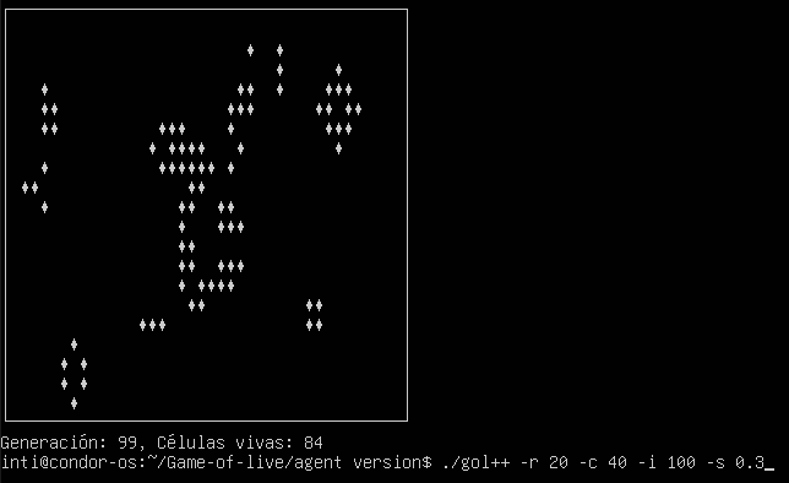
\includegraphics[width=0.40\columnwidth]{figures/gol-demo.png}
                \caption{Ejemplo de funcionando del programa Juego de la Vida.}
                \label{fig:gol-demo}
            \end{figure}
            
        \end{addmargin}
        
    \end{enumerate}


    \subsection{Análisis condiciones mínimas}


    Todo sistema operativo y todo sistema de software tiene condiciones mínimas de operación. Determine la cantidad mínima de memoria RAM que necesita Ubuntu 24.04 para funcionar normalmente. Lo anterior, para esta trabajo, significa que tanto el sistema operativos y los programas compilados se pueden ejecutar sin problemas.

    

\end{document}